\documentclass{article}
\usepackage{fullpage}
\usepackage{amsmath,amssymb}
\usepackage{natbib}
\usepackage{marginnote}
\usepackage{graphicx}
\usepackage{hyperref}
\usepackage{latexml} % for \iflatexml

\newcommand{\var}{\mathop{\mbox{Var}}}
\renewcommand{\P}{\mathbb{P}}
\newcommand{\E}{\mathbb{E}}
\newcommand{\R}{\mathbb{R}}

\bibliographystyle{plain}

\begin{document}

\section{Introduction}

Recall questions of origin of adaptations

Reference on parallel adapation, standing variation, etc.:
  coop,
  pennings and hermisson,

Summarize previous paper

Question assumptions of no standing variation and homogenous selection

Stick to constant-speed waves.

\section{General model}

outline here assumptions common to both models.

\section{Standing variation}

\subsection{The set-up}

% selection pressure changes at $t=0$ from $1-s_d$ to $1+s_b$ -- homogeneous

For now we ignore geographic hetergeneity, and assume that the species range
is a homogenous, one- or two-dimensional region. 
There are two selective classes -- the {\em neutral} type, and the {\em mutated} type.
We assume that different mutations are distinguishable --
either as selectively equivalent mutations, or by linked variation.
For a long time in the past, the mutated type has been at a selective disadvantage (long enough to be at selection-mutation equilibrium),
but at a certain time the selective regime changes, so that the mutated type has a selective advantage and quickly spreads to fixation.
After fixation, alleles are either descended
from families of mutants present as standing variation when the selective regime changed,
or from new mutants arising since that time.

For concreteness, suppose that before time $t=0$,
the mutant type has fitness $1-s_d$ relative to the neutral type
(i.e.\ it produces on average $1-s_d$ times the number of offspring per generation),
and that after time $t=0$,
the mutant type has fitness $1+s_b$,
where $s_b>0$ will usually be assumed to be small, and $0<s_d<1$.
We assume that diploid fitness is additive, or at least that the important dynamics are determined by the haploid fitness.
The number of offspring has finite variance, which to keep the formulas simple we assume to be equal to one.
(If the mutation is recessive, XXX more complicated things happen.)
As for the other parameters,
suppose that each offspring of a neutral parent is of the mutant type with probability $\mu$,
and that the mean squared distance between parent and child is $\sigma^2$ (the {\em dispersal variance}).
The species occupies an area with mean density
$\rho$ haploid individuals (or chromosomes) per unit area.
\marginnote{XXX or do diploid? below is haploid.}

% Branching-process-sized point mass approx to local groups present at $t=0$
% -- depends on local population density large enough relative to migration (to be "branching")
% -- and migration not too large (since we approximate as a point mass).
% Find mean density of clusters of successful standing mutants. 
% Is greater-than-one size of clusters likely to make a difference? 

We make use of the commonly used approximation that neglects competition between relatives,
treating the offspring of a new mutant that appears in an area not already occupied by the mutated type
as a branching process.
After $t=0$, the offspring of a single mutant form (approximately) a branching process with growth rate $s_b$,
so each new mutant establishes locally with probability $p_s \approx 2s_b$.
As in \cite{ralphcoop2010}, each new offspring has a very small probability of being a mutant and establishing locally,
so the collections of times and locations at which mutants appear and establish locally 
is well--approximated by a Poisson process in space and time.
This the rate of this Poisson process, 
the rate per unit area at which new mutants appear and establish locally after $t=0$ in areas not already occupied by the mutant type
is approximately $\lambda = 2 \mu \rho s_b$.

Before $t=0$, on the other hand, the mutation is deleterious, so the genetic descendents of each new mutation are (with high probability) doomed to extinction,
but may persist for some time.
Since the times and locations of mutants before $t=0$ also well-approximated by a Poisson process with rate $\mu \rho$,
the locations of all mutant families extant at $t=0$ whose descendents are destined to fix locally is also,
by the Mapping theorem, a Poisson process with rate we define to be $\lambda_0$.
If we assume that the descendants of at most only a few members of any extant mutant family at $t=0$ will survive,
and that these progenitors are near to each other in space, we can then treat each such family as a single mutant,
equivalent to the mutants arising later.
(The approximation will be good if the log of the size of an extant families is small relative to the establishment time,
and the spatial distribution of the family is small relative to the spread between them.)
To find $\lambda_0$, consider a mutation that arose at time $-T<0$, and let $Z_s$ be the number of its descendants at time $s-T$.
At time $t=0$, there are $Z_T$ individuals present with the mutation,
and each has probability $p_s \approx 2s_b$ of establishing, approximately independently.
Therefore, the probability that some descendants of this mutation establish and fix locally is $1-(1-p_s)^{Z_T}$,
so defining $\zeta(u,t) = \E[u^{Z_t} | Z_0=1 ]$ to be the generating function of $Z_T$,
the rate is
\begin{align*}
    \mu \rho \int_0^\infty \left( 1- \zeta(1-p_s,T) \right) dT .
\end{align*}
Now for $s_b$ small, using $p_s \approx 2s_b$ and that $\E[Z_T]=(1-s_d)^T$,
we know that $\zeta(1-2s_b,T) \approx 1-2s_b \E[Z_T] = 1-2s_b (1-s_d)^T$,
resulting in the approximation
\begin{align}
    \lambda_0 &= \mu \rho \int_0^\infty 2s_b (1-s_d)^{T} dT \\
        &= \frac{ 2 \mu \rho s_b }{ -\log(1-s_d) } .
\end{align}

XXX More discussion on whether this is a good approximation?  
Compute typical size and radius of a standing cluster?

recall PPP computations; draw cones of opportunity for new mutations 

\subsection{Characteristic parameters}

% a characteristic length of regions and a proportion of haplotypes (or of space?) that are from standing variation

In \citet{ralphcoop2010}, studying the model without standing variation,
we defined a {\em characteristic length} which gave the spatial scale across with mutants with distinct origins would establish.
This was proportional to the mean distance between neighboring established mutants,
but had the advantage of being easier to calculate.
Furthermore, the time scale over which adaptation occurred could be found by dividing the characteristic length 
by the speed at which the mutants spread.
We will define the characteristic length for this model,
as well as a similar compound parameter describing the relative importance of standing variation to the process of adaptation.
(Note that a similar approach, summarizing with a {\em characteristic length} was taken by \citep{slatkin1973geneflow} for a different problem.)

Suppose we fix our attention on a particular new mutation that happens to be the first to occur in some region.
As it spreads, it will cover a distance $L$ in time $L/v$, where $v = \sigma \sqrt{2s_b}$ is the speed of the wave of advance.
The number of other mutations appearing in the circle it has covered up until this time is Poisson with mean
$\lambda_0 \pi L^2 + \lambda \pi L^3 /v$ in two dimensions
(and $\lambda_0 2 L + \lambda \pi L^2 /v$ in one dimension).
% $\lambda_0 \omega_d L^d + \lambda \omega_d L^{d+1} /v$ in $d$ dimensions
Therefore, if we define $\chi$ to be the unique positive solution to
\[
    \lambda_0 \pi \chi^2 + \lambda \pi \chi^3 /v = 1,
\]
then $\chi$ gives the distance spread unobstructed by the descendants of a new mutant
before it is expected that one other successful mutation would have arisen in the area covered so far.
The explicit formula for $\chi$ is cumbersome; here we omit it.
(This is in two dimensions; in one dimension the characteristic length is $\chi = \frac{ \sqrt{ 4 \lambda_0^2 + 2\lambda v } - 2 \lambda_0 }{ 4 \lambda v }$.)
This can be rewritten 
\begin{equation} \label{eqn:defines_chi}
%    \left( \frac{ - \chi \log(1-s_d) }{ 2 s_b \sigma } \right)^2 + \left( \frac{ - \chi \log(1-s_d) }{ 2 s_b \sigma } \right)^3 
%        = \frac{ - \log(1-s_d)^3 }{ 4 s_b^2 \sigma^2 \pi \rho \mu } .
   \frac{\sqrt{2s_b} }{-\log(1-s_d) } \chi^2 + \frac{1}{\sigma} \chi^3 = \frac{1}{\sqrt{2s_b} \rho\mu\pi}
\end{equation}
From this we see that $\chi$ decreases with $\rho$ and $\mu$.
Furthermore, for large $\sigma$, the characteristic length is close to the value obtained just from standing variation:
$\chi = \sqrt( -\log(s_d) / 2 s_b \rho \mu \pi ) + O(1/\sigma)$.
On the other hand, if the mutant allele is highly deleterious before $t=0$,
then the characteristic length is close to the value from \citet{ralphcoop2010}:
$\chi = ( \sigma / \rho \mu \pi \sqrt{2 s_b} )^{1/3} + O(1/\log(1-s_d))$.

XXX could do calculations as in "panmixia" here, e.g. if $f = (\chi/\sqrt{\pi \lambda_0})^2$ then
$f = 1-\gamma f^{3/2}$, where
$\gamma = (4 \pi^{5/2} / \sqrt{2}) \mu^2 s_b^{3/2} \rho^2 / \sigma \log(1/(1-s_d))$.
Then if $\gamma \ll 1$, $f \approx 1$, while if $\gamma \gg 1$, then $f \approx 0$.

By the above calculation, we know that the relevant mutations occur about distance $\chi$ apart, 
and occur within the first $\chi/v$ generations.
Said another way, if we look in a circular region of space of radius $\chi$ over $\chi/v$ generations,
we expect to find one mutational origin;
we denote the probability that this mutation is from standing variation by $\pi_0$.
Therefore, $\pi_0$ is roughly the proportion of establishing mutations that come from standing variation,
and it is an elementary consequence of the Poisson process that
\begin{align} \label{eqn:pizero}
    \pi_0 = \lambda_0 \pi \chi^2 .
\end{align}
\marginnote{put in value of $\chi$ computed above.}
(In one dimension, $\pi_0 = 2 \lambda_0 \chi$.)

\subsection{Standing Variation -- Results} 

The quantity that is perhaps easiest to compute is the mean time until adaptation.
Fix some geographic location, and let $\tau\ge0$ be the time at which the point is reached by the advantageous mutations.
Then, as shown in Figure XX,
$\tau > t$ if and only if the cone with point at $(x,t)$ and slope $v$ extending back to $t=0$ is empty of successful mutations.
Since we assume these are a Poisson process, 
\[
    \P\{ \tau > t \} = \exp\left( - \lambda_0 \pi v^2 t^2 - \lambda \pi v^2 t^3 / 3 \right) ,
\]
and so we have
\begin{align}
    \E[\tau] % &= \int_0^\infty \P\{ \tau > t \} dt \\
        &= \int_0^\infty \exp\left( - \lambda_0 \pi v^2 t^2 - \lambda \pi v^2 t^3 / 3 \right) dt.
\end{align}
For means of evaluting this integral, see Appendix \ref{apx:integrals}.

% proportion of haplotypes (and of space) that are from standing variation 

We have defined $\lambda_0$ to be the mean density of standing variants that reach local fixation.
Define $\nu_+$ to be the mean density of new mutants whose offspring fix locally.
Since the probability that a mutant arising at $(x,t)$ is lucky enough to be born in a location not already occupied by mutants
is $\P\{ \tau > t \}$,
we can see  $\nu_+ = \int_0^\infty \lambda \P\{\tau>t\} dt$, and hence
$\nu_+ = \lambda \E[\tau] $.
Using that $\lambda_0 = \lambda / \log(1/(1-s_d))$, this gives us that
\begin{equation}
    \nu_+ = (\mbox{mean density of new patches}) = \frac{1}{1-\log(1-s_d) \E[\tau]} .
\end{equation}
Since the mean proportion of patches that come from standing variation is $\lambda_0 / (\lambda_0 + \nu_+)$,
this gives us the exact quantity we approximated by $\pi_0$ in \eqref{eqn:pizero}.
There are $\lambda_0 + \nu_+$ patches per unit area, so
the typical patch (i.e.\ with distribution given by the Palm measure) occupies area $1/(\lambda_0 + \nu_+)$.

We can also find the mean proportion of space covered by standing variants.
If by time $t$ a geographic location has not yet been reached by the mutation,
the probability it will be reached by time $t+dt$ 
by a standing variant is approximately $2 \lambda_0 \pi v^2 t dt$, 
and the probability it is reached by a new variant is $\lambda \pi v^2 t^2 dt$.
Therefore, as is standard for competing exponentials,
the probability a given location is reached first by a standing variant,
and therefore the mean proportion of space covered  by standing variants,
is
\begin{equation}
    z_0 = \int_0^\infty {2 \lambda_0 \pi v^2 t} \; \exp \left( - \lambda_0 \pi v^2 t^2 - \lambda \pi v^2 t^3 / 3 \right) dt .
\end{equation}
\marginnote{put in this value in terms of Gaussian CDF?}
To evaluate this integral, again see Appendix \ref{apx:integrals}.

Furthermore, if we define $a_0$ to be the mean area occupied by a typical standing variant, 
then $a_0$ is given by the proportion of the range occupied by standing variants over the mean density of unique standing variants,
i.e.\ $a_0 = z_0 / \lambda_0$.
We can compare this to the corresponding quantity $a_+$ for a new variant through the formula
$a_0 / a_+ = z_0 / (1-z_0)$.

\begin{figure}[ht]
\begin{center}
\includegraphics[width=1.0\textwidth]{charlen-by-sd-limit.eps}
\caption{ %
{\bf Characteristic length,} as a function of selective disadvantage, compared to the corresponding quantity without standing variation (e.g.\ from \cite{ralphcoop2010}) and to the quantity only considering standing variants (e.g.\ $\sqrt{\lambda_0}$).
}
\end{center}
\end{figure}

\begin{figure}[ht]
\begin{center}
\includegraphics[width=1.0\textwidth]{proportion-by-sd.eps}
\caption{ %
{\bf Mean proportion of patches arising from standing variation.} The paramters given are for the sickle-cell example.  XXX say more.
}
\end{center}
\end{figure}

\begin{figure}[ht]
\begin{center}
\includegraphics[width=1.0\textwidth]{charlen-by-sd-sigma.png}
\caption{ %
{\bf Characteristic length,} as a function of dispersal distance $\sigma$ and selective disadvantage $s_d$.  XXX at what parameters. XXX
}
\end{center}
\end{figure}

\marginnote{do mean (and variance?) of distance between haplotypes?}

influence of migration on things -- plot these versus migration 

{\tt Simulations:} compare mean density against $s_d$ at different values of $\sigma$; omit variability if needed for readability.
Compare to panmictic results.


\section{Local establishment}

Include stuff from ``comparison to panmixia'' here:

Note that we are not considering the time it takes the mutation to fix locally.  
How long is this time?  Mean, variance.
When would we expect more mutations in this time?
Roughly, if populations are larger than $C/\mu$ for some $C \approx 100$.

Both these results and the panmictic calculations are underestimates.  
If the time to local fixation is enough to change things significantly, 
we are in the realm where the panmictic results apply better.

Graph: sigma against mean number of origins; different curves for spatial, panmictic (flat), and simulation;
different values of theta as different line types?
Mention Monty's empirical speeds paper.

Compare to panmixia: increases degree of parallel mutation if... ?
Check P and H papers and Orr and Betancourt.  (standing variation only)

\section{Patchy selection} 
\label{ss:discretedemes}

We have been working in a continuous model of geographic space; 
in this section we move to a discrete model of isolated populations exchanging rare migrants,
but in section \ref{ss:patchyspace} discuss how a model with {\em patchy} selection can be approximated by such a discrete model.

Suppose now that we have a set of $L$ discrete populations of individuals that may reproduce or migrate,
and that migration and mutation are rare, so that the waiting times until either event is approximately exponential.
Suppose that for each pair of populations, labeled $i$ and $j$, the mean number of migrants that travel from $i$ to $j$ per generation
is $M_{ij}$ and that the mean number of new mutations appearing in population $i$ per generation is $\mu_i$.

{\tt Include cartoon here.}

If we suppose that fixation occurs on a faster time scale than mutation or migration,
so that it is very unlikely that two different migrants or mutants begin to fix locally in the same population,
then we can treat the process of extinction or local fixation as instantaneous 
(a limit previous studied by \cite{Slatkin:81}).
In this limit we may also ignore swamping effects of inmigration of nonmutant alleles.

In this case, we have the following picture.
The population at first starts out with no selected alleles. 
At some later time point suppose that there are $T$ different alleles present in the population, 
that the $k^\mathrm{th}$ allele is occupying demes $\{i^k_1, \ldots, i^k_{n_k}\}$, for $1\le k \le T$.
Let $I$ denote the set of all adapted demes, 
and let $J = \{j_1, \ldots, j_\ell\}$ denote the demes that have not yet adapted, with $\ell = L - \sum_k n_k$.
Then we are assuming that two types of event can happen which could change the state:
either at rate $\mu_j p_f$, an unadapted deme $j$ produces a new mutant, which fixes in this deme;
or at rate $M_{ij} p_f$, an adapted deme $i$ sends a migrant to unadapted deme $j$, which fixes in that deme.
Therefore, under these assumptions, the probability of fixation $p_f$ (and hence the selection coefficient)
only enter as a time scaling: for instance,
if we define $R = \sum_{j \in J} \left( \mu_j + \sum_{i \in I} M_{ij} \right)$,
then the total rate of such events is $p_f R$.
The probability that the next event results in, say, adaptation of deme $j$
is 
\[
 \left( \mu_j + \sum_{i \in I} M_{ij} \right) / R,
\]
and the probability that deme $j$ adapts through migration from deme $i$, given that deme $j$ is the next to adapt, is
$M_ij / R$,
while the probability that it adapts through a new mutation is $\mu_j / R$.

The main point here is that the final pattern,
and hence the likely extent of parallel adaptation,
is independent of the strength of selection.
This is in contrast to the continuous case, however, this observation is dependent on the assumption of weak migration
and fails to hold if different migrant lineages interact.
This can be viewed as a continuous-time Markov process XXX.
Explicit solutions are not available in the general case,
but if we specialize to a completely symmetric model (i.e.\ the ``island'' model),
then the mathematical picture is a pretty one.

\subsection{Symmetric patches}

Indeed, suppose that migration and mutation are symmetric: $M_{ij}=m$ and $\mu_j = \mu$ for all $j$ and $i\neq j$.
Suppose at some time the $k^\mathrm{th}$ allele is occupying $n_k$ demes, 
with $n = \sum_k n_k < L$.
Then at rate $(L-n) N \mu p_f + n (L-n) N m p_f$,
either a migration or mutation event happens.
With probability $\mu/(\mu + n m)$, it is a mutation,
and a new deme is randomly chosen and assigned a new allele.
With probability $n_k m / (\mu + n m)$,
the $k^\mathrm{th}$ type sends a successful migrant to a randomly chosen new island,
which is assigned the $k^\mathrm{th}$ allele.

This process is a continuous-time version of the ``Chinese restaurant process''
described in \citet{aldous1985exchangeability} and \citet{pitman1995partitions},
and so the final partition of types across demes has the Ewens sampling distribution with parameter $\mu/m$.
Again note that the selection coefficient, which is implicit in the probability $p_f$,
does not enter into the final distribution.

Now we can compute most properties we might want about the process.
For instance, the expected number of distinct mutational origins is
\begin{equation}
    \E\left[ \mbox{ \# of independent mutations } \right] = 
            1 + \frac{\mu}{m} \sum_{k=2}^L \frac{1}{k+(\mu/m)}. \label{discrete_expected}
\end{equation}
The probability that there is only a single successful mutation is
\begin{equation}
\P \left\{ \mbox{only one mutational origin} \right\} = 
            \prod_{k=1}^{L-1} \frac{ k }{ k+(\mu/m)} .
\end{equation}
More generally, suppose we sample a single deme, and are interested in the total number of demes $S$
(including the sampled one) that share the same fixed mutation as our sampled deme.
Then $S$ has distribution
\begin{equation} \label{eqn:Sdistrn}
\P\{ S=s \} = \frac{ (s-1)! (\mu/m)^{L-s} }{ \prod_{k=1}^{L-1} (k+(\mu/m)) } .
\end{equation}
Furthermore, if $L$ is large, then $S/L$ has probability density approximately
\begin{equation} \label{eqn:betadistrn}
   (\mu/m) (1-x)^{(\mu/m)-1}
\end{equation}
namely, is a $\mathrm{Beta}((\mu/m), 1)$ distribution--- see \cite{donnelly-joyce} and \cite{permanPitmanYor92}.

% In Figure \ref{fig:discbyratio} we plot mean number of types and size (number of demes occupied) of a sampled type,
% for a model with 20 interconnected demes, across different parameter values.  
% This indicates that we need the population-scaled mutation and migration rates to be within a factor of about 100 of each other for parallel adaptation to leave an interesting pattern. If migration is faster, then a single type is likely to take over, while if migration is weaker, each deme is likely to come up with its own type.

The high connectedness of the discrete deme island model means that the expected number of distinct alleles, (Equation \eqref{discrete_expected}), 
grows with the $\log$ of the number of demes. This strongly contrasts with the continuous spatial model where the local nature of dispersal means that doubling the species range will double the number of mutations expected. 
Furthermore, while in the continuous model the areas occupied by distinct mutations are similar in area, in this strong-selection discrete island model, 
only a few types tend to dominate even as the number of demes (and thus, distinct types) grows large (see Equations \eqref{eqn:Sdistrn} and \eqref{eqn:betadistrn}).

A more general model would allow migration only along edges of some graph connecting the demes.
In the low migration limit such a model still produces a partition distribution independent of the selection coefficient,
but it does not in general have the Ewens distribution.
Another extension would be to include the time alleles need to achieve an intermediate frequency,
along the lines of \citet{Navarro:03}, which would reintroduce dependence on the selection coefficient.

\texttt{XXX omit this? XXX}
We have treated the time during which the selected allele is at intermediate frequency in a deme (about $\log(\sigma^2 \rho)/s_b$ generations) as negligible, 
which ignores migration events that occur while the mutation is spreading through the population. 
we now sketch of a more realistic approximation.
For each occupied--unoccupied pair of demes, if the number of mutant alleles in the occupied deme is $n(t)>0$,
then at time $t$, migrants from the occupied deme pass the selected allele to the unoccupied deme at rate $2 n(t) m p_f(s_b)$,
while newly arisen mutants arise and fix in the unoccupied deme at constant rate $2 N \mu p_f(s_b)$.
The selected type should grow approximately as $n(t)=\exp(s(t-t_0))$.
Of course, to follow this model through, we will have to account for multiple types within a single deme and other complications,
but we can at least make a few observations.
One is that the final distribution of types is no longer independent of $s_b$, which enters through the dynamics $n(t)$.
However, it is clear that increasing the selection coefficient $s$ will decrease the number of types (independent mutational origins),
while on the other hand, increasing the deme size $N$ will increase the number of types,
and that the case presented above is at the extreme (see also \cite{Navarro:03} for deterministic approximations). 


\subsection{Relation to a continuous model
\label{ss:patchyspace}

A similar situation of interest is the case when the species occupies a continuous range, but the selective pressure itself is patchy.
If the areas where the new allele is advantageous are relatively isolated,
we might hope to apply the results above to such a situation.
For this purpose, suppose that instead of a uniform habitat,
the selective pressure is such that the new alleles are only advantageous in isolated locations, 
and are disadvantageous in the intervening region.
As before, we assume that the new allele has fitness $1+s_b$ relative to the unmutated type in the ``good'' patches,
and assume that it has fitness $1+s_m$ in the intervening areas, with $s_m<0$.
To make things tractable, we assume that the distances between the patches are large relative to migration distance $\sigma$,
and that the disadvantage $s_m$ ensures that on the relevant timescale,
the allele is very unlikely to fix locally in the regions where it is at a disadvantage.
With these assumptions as justification, we will move to a model of discrete demes exchanging migrants,
where ``migration'' occurs through the rare, transient passage of the new allele through regions where it is disadvantageous.

equal deme sizes?  general migration rates?

\subsubsection{Mutational influx}
\label{ss:patchymutation}

Consider first a single, isolated patch of area $A$ in which no new allele has appeared.
\citet{barton1987establishment} (or \citet{slatkin1973geneflow}?) has studied this situation (in one dimension)
and found that:
mutations appearing further than a few multiples of $\sigma/\sqrt{2s_m}$ away from the patch have vanishingly small probability of establishment;
mutations appearing within the patch have probability strictly less but approaching that $2s_b$ of establishment;
and if the patch width is less than $2 \tan^{-1} (\sqrt{s_m})$, then local fixation does not occur (rather, is not stable).
Let $p(x)$ be the probability that a new allele arising at location $x$ fixes.
The function $p(x)$ can be found in terms of Jacobi elliptic functions,
XXX as shown in the Appendix,
but the expressions are particularly unhelpful.
The total successful mutational influx per generation is then given by $\int \rho \mu p(x) dx$,
and depends in a complicated way on the relationship of patch width and selection coefficients,
but still scales linearly with the population mutational influx $\rho \mu$.
Therefore, we define $p_f = \int p(x) dx$, and in a pinch will approximate this by $2 s_b A$,
which will be a good approximation if the width $\sqrt{A}$ is large relative to $\sigma/\sqrt{2s_m}$.

XXX We are interested in the case where a single mutation only takes over? XXX

\subsubsection{Migration rates}
\label{ss:patchymigration}

Now suppose that there are two patches, each of area $A$, of good environment separated by distance $R$,
and that the allele has begun to fix in the first, but has not yet appeared in the second.
As above, any copy of the new allele that appears at location $x$ relative to the second, unadapted patch 
has probability approximately $p(x)$ of fixing locally in this patch,
whether the allele is a new mutation or is descended from the occupants of the first patch.
Due to mutation--selection balance there will be a small number of alleles descended from those of the first patch (``migrants'') 
present in the regions where they are disadvantageous;
the equilibrium frequency may again be expressed in terms of Jacobi elliptic functions (Appendix XXX, citeXXX),
although the equations are again not particularly helpful.
However, we do know that if $q(r)$ is the expected proportion present at mutation--selection balance at distance $r$ from the first patch
in the absence of the second patch, that for large $r$ the proportion decays exponentially, $q(r) \approx C \exp( -|\sqrt{s_m} r / \sigma|)$,
where $C$ is a constant depending on the structure of the populations and the selection coefficients.

Combining this with the calculations above allows us to get a rough sense of the scale of migration between separated patches,
supposing that patches are large enough for local fixation to be stable.
If the alleles were not advantageous in the second patch,
the average numbers of mutant alleles present near the second patch would be around $\rho A \exp( - |\sqrt{s_m} R/\sigma| )$;
so the waiting time until some migrant allele fixes in the second patch would be something like $T_m = ( 2 s_b \rho A \exp( - |\sqrt{s_m} R/\sigma|)^{-1}$.
If $T_m$ is large, then we would expect successful migrants to be rare,
so that if the second patch adapts through migration, it is likely to come from only a single migrant.
We leave aside the converse situation, for which there is likely to be more than one migrant
that founds the population mutant individuals in the new patch.


\subsection{Patchy Selection -- Results} 
\label{ss:discreteresults}

If environment is continuous, with separated patches where the new allele is advantageous,
we can only get a rough sense of whether the new adaptation is likely to spread through mutation (i.e.\ in parallel)
or through migration.
Taking the expressions from sections \ref{ss:patchymutation} and \ref{ss:patchymigration} above,
we see that if patches each have sufficiently large area $A$,
then the mutational input in each is on the order of $2 \rho \mu A$,
while the influx due to migration between patches separated by distance $R$ is on the order $2 \rho A \exp(- |\sqrt{s_m} R/\sigma|)$. 
If the input from mutation and migration are comparable, i.e.\ if $\mu \approx \exp( -|\sqrt{s_m} R/\sigma| )$,
then adaptation is expected to take place both by migration and mutation.
If we take $\mu = 10^{-8}$, then this is satisfied if $R/\sigma \approx 18/\sqrt{s_m}$.
so if the disadvantage to the new mutation between patches is fairly strong (say, $s_m=.05$),
then the distance between patches must be about a hundred times the dispersal distance (i.e.\ $R/\sigma \approx 100$);
while if $s_m$ is much smaller, say $s_m = .001$, 
then the patches must be separated by many hundreds of times the dispersal distance (i.e.\ $R/\sigma \approx 500$).
The situation does not change much if $\mu$ is larger -- even if $\mu = 10^{-6}$, 
the required separation between patches is only reduced by 60\%.
If the separation between patches is much larger -- say, by a factor of ten -- 
then patches are effectively isolated -- most adaptation will be independent between patches.
On the other hand, if the separation is much smaller, then a single mutation is likely to fix everywhere.

Furthermore, in the model of discrete demes connected by symmetric weak migration, 
the final distribution of types depends only on the ratio of mutation to migration rates,
and that the number of independently arisen types follows the Ewens distribution, with parameter $\mu/m$.
In Figure \ref{fig:discbyratio} we plot mean number of types and size (number of demes occupied) of a sampled type,
for a model with 20 interconnected demes, across different parameter values.  
This indicates that we need the population-scaled mutation and migration rates 
to be within a factor of about 100 of each other for parallel adaptation to leave an interesting pattern.  
If migration is faster, then a single type is likely to take over, while if migration is weaker, each deme is likely to come up with its own type.

\begin{figure}[ht]
 \begin{center}
 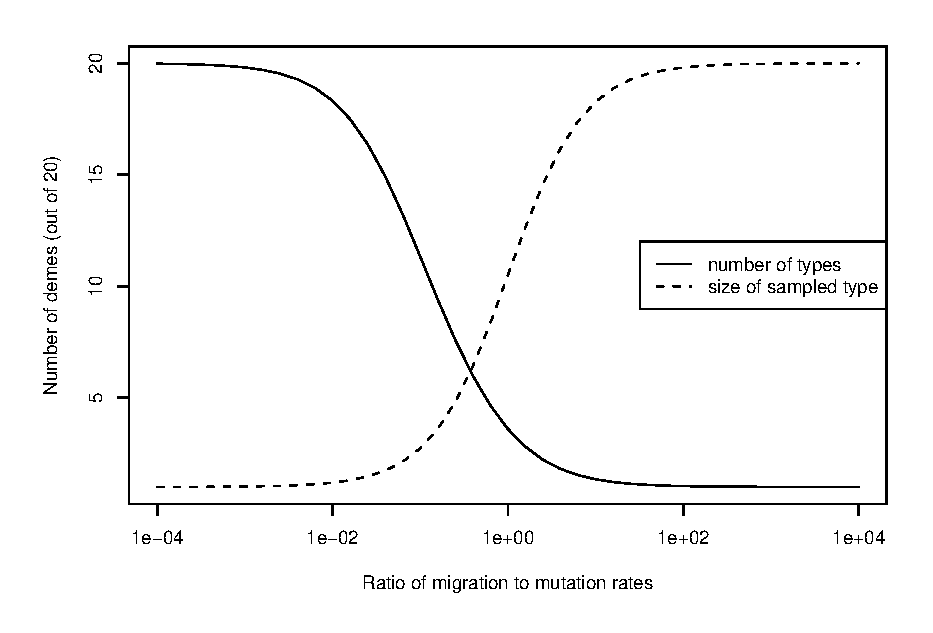
\includegraphics{discrete-by-ratio.eps}
 \caption{ %
 The mean number of types and the mean number of demes occupied by a sampled type, in a discrete model with 20 demes,
 plotted as a function of the ratio of migration to mutation probabilities.
 Note the log scale on the horizontal axis.
 \label{fig:discbyratio}
 }
 \end{center}
\end{figure}

Also note that the properties of the discrete model are independent of the {\em sizes} of the demes themselves--- we have assumed away all such dependence.
This is complementary to the results of \cite{softsweepsII}, who showed that multiple mutations are likely to arise {\em within} a panmictic deme
if the population-scaled mutation rate $2 N \mu$ is greater than $1$.

\section{Applications} 

HbS

lava bed peromyscus

G6PD

\section{Discussion} 

if populations and mutation rates are large enough, parallel adaptation is likely, aided by geography. 
recall others' work. 

patchy selection helps this happen; 
effective migration rate looks like what; 
strength of (positive?) selection suprisingly does not affect results (?) 

standing variation will be important under these circumstances; 
migration rate (and so geographic structure) will not affect numbers of types if this is true; 
however migration always affcts spatial patterns. 

discussion of applications. 

discuss mixing of types; 
Graph: from simulation showing local proportions in a single patch showing initial fixation of a single type and later mixing converging toward more than one type.  (and eventual loss of one?)

\bibliography{standing_patches_refs}

\appendix

\section{Integrals appearing in the text}
    \label{apx:integrals}

In the text at several points appear integrals of the form
\begin{align}
  \int_0^\infty t^c \exp \left( - \alpha t^d - \beta t^{d+1} \right) dt 
\end{align}
where $c$ is a positive integer, $d$ is the dimension, and $\alpha$ and $\beta$ are positive real numbers.
This could be evaluated through standard numerical methods; below we describe a power series expansion.
Changing variables to $u = \beta t^{d+1}$, this becomes
\begin{align}
    \left( (d+1)^{-1} \beta^{ (1-c)/(d+1) } \right) \int_0^\infty u^{(c+1-d)/(d+1)} \exp\left( - \alpha \beta^{-d/(d+1)} u^{d/(d+1)} - u \right) du ,
\end{align}
so it suffices to evaluate the function
\begin{equation}
    G(a,b,x) := \int_0^\infty  t^a \exp\left( -x t^b - t \right) dt ,
\end{equation}
in the case that $a=(c-d+1)/(d+1)$, $b=d/(d+1)$, and $x$ is a function of the demographic paramters.
Since $a$ and $b$ only depend on the dimension and the quantity being computed,
we are interested in $G$ as a function of $x$.
At least in the case $b=d/(d+1)$ it is possible to express $G$ as a finite sum of gamma functions,
but we proceed with a simpler method.
Note that $\partial_x G(a,b,x) = -G(a+b,b,x)$,
and that at $x=0$, the function $G$ is the gamma function $G(a,b,0) = \Gamma(a+1)$.
Therefore, a Taylor series for $G$ would be
\[
    G(a,b,x) = \sum_{n \ge 0} = \sum_{n \ge 0} \frac{(-x)^n}{n!} \Gamma(a+nb+1) .
\]
It is easy to check using Stirling's formula that $\limsup_{n \to \infty} ( x^n \Gamma(a+nb+1)/n! )^{1/n} = 0$
if $b<1$, so the sum converges.

\end{document} 
